\chapter{Числовые и степенные ряды}\markright{Глава 30}

\section*{Бесконечная сумма и её частичные суммы}
\begin{definition}
\term{Числовой ряд} (\emph{numerical series}) \(\sum_{n=1}^\infty a_n\) изучается через \par \term{частичные суммы} (\emph{partial sums}) \(S_N=\sum_{n=1}^N a_n\). Ряд \par \term{сходится} (\emph{converges}), если \(S_N\) имеет конечный предел \(S\); этот предел называется суммой ряда. В остальных случаях ряд расходится.
\end{definition}
\par\addvspace{5pt}\begin{lrbox}{\CatFlowBox}\begin{minipage}[t]{\linewidth}
\setlength{\parskip}{5pt}\setlength{\columnsep}{4.5mm}\setlength{\intextsep}{0pt}
\begin{wrapfigure}[11]{r}{54mm}

\includegraphics[width=54mm,height=58mm,keepaspectratio]{images/unique/art-126.png}
\end{wrapfigure}
Запись бесконечной суммы требует отдельной проверки сходимости. Слагаемые могут становиться маленькими, а общий итог всё равно расти без ограничения. Полезно каждый раз возвращаться к конечной сумме \(S_N\), оценивать её и лишь затем переходить к пределу. Обычные действия с бесконечными выражениями оправдываются такими оценками.
\par\WFclear\end{minipage}\end{lrbox}%
\ifdim\dimexpr\ht\CatFlowBox+\dp\CatFlowBox\relax<64mm\dp\CatFlowBox=\dimexpr64mm-\ht\CatFlowBox\relax\fi%
\noindent\usebox{\CatFlowBox}\par\addvspace{5pt}
\begin{theorem}[Необходимое условие сходимости]
Если ряд \(\sum a_n\) сходится, то \(a_n\to0\). Обратное утверждение неверно.
\end{theorem}
\par\addvspace{5pt}\begin{lrbox}{\CatFlowBox}\begin{minipage}[t]{\linewidth}
\setlength{\parskip}{5pt}\setlength{\columnsep}{4.5mm}\setlength{\intextsep}{0pt}
\begin{wrapfigure}[13]{l}{54mm}

\includegraphics[width=54mm,height=58mm,keepaspectratio]{images/unique/art-129.png}
\end{wrapfigure}
\textit{Доказательство.} При \(n\ge2\) имеем \(a_n=S_n-S_{n-1}\). Если обе частичные суммы стремятся к \(S\), разность стремится к нулю. Контрпример к обратному утверждению — гармонический ряд, расходимость которого докажем ниже.\hfill\(\blacksquare\)
\par\WFclear\end{minipage}\end{lrbox}%
\ifdim\dimexpr\ht\CatFlowBox+\dp\CatFlowBox\relax<64mm\dp\CatFlowBox=\dimexpr64mm-\ht\CatFlowBox\relax\fi%
\noindent\usebox{\CatFlowBox}\par\addvspace{5pt}

\begin{theorem}[Критерий Коши для ряда]
Ряд с действительными членами сходится тогда и только тогда, когда
\[
\forall\varepsilon>0\ \exists N\ \forall m>n\ge N:
\left|\sum_{k=n+1}^{m}a_k\right|<\varepsilon.
\]
\end{theorem}
\begin{proof}
Сумма в модуле равна \(S_m-S_n\). Условие означает, что последовательность частичных сумм является последовательностью Коши. Применяем полноту \(\mathbb R\) из главы 28.
\end{proof}
\section*{Ряды с неотрицательными членами}
\begin{theorem}[Ограниченность частичных сумм]
Для \(a_n\ge0\) ряд сходится тогда и только тогда, когда его частичные суммы ограничены сверху.
\end{theorem}
\begin{proof}
Частичные суммы не убывают. Если они ограничены, применяется теорема о монотонной последовательности из главы 12. Обратно, сходящаяся последовательность ограничена.
\end{proof}
\begin{theorem}[Признак сравнения; comparison test]
Пусть начиная с некоторого номера \(0\le a_n\le b_n\). Если \(\sum b_n\) сходится, то \(\sum a_n\) сходится. Если \(\sum a_n\) расходится, то \(\sum b_n\) расходится.
\end{theorem}
\begin{proof}
Удаление конечного числа первых членов не влияет на сходимость: частичные суммы меняются на одну постоянную. Для оставшихся членов частичные суммы меньшего ряда не превосходят частичных сумм большего. Ограниченность большого ряда влечёт ограниченность малого. Второе утверждение — контрапозиция первого.
\end{proof}
\begin{theorem}[Гармонический ряд; harmonic series]
Ряд \(\sum_{n=1}^\infty\frac1n\) расходится, хотя \(\frac1n\to0\).
\end{theorem}
\begin{proof}
Сгруппируем члены от \(2^{k-1}+1\) до \(2^k\), \(k\ge1\). В группе \(2^{k-1}\) слагаемых, каждое не меньше \(2^{-k}\), поэтому сумма группы не меньше \(\frac12\). Следовательно, \(S_{2^m}\ge1+\frac m2\to+\infty\).
\end{proof}
\begin{theorem}[Степенные числовые ряды; p-series]
Для действительного \(p\) ряд \(\sum_{n=1}^\infty\frac1{n^p}\) сходится тогда и только тогда, когда \(p>1\).
\end{theorem}
\begin{proof}
При \(p\le0\) члены не стремятся к нулю. При \(0<p\le1\) они не меньше \(\frac1n\), поэтому ряд расходится по сравнению с гармоническим.
Если \(p>1\), в группе \(2^k\le n<2^{k+1}\) имеется \(2^k\) членов, каждый не больше \(2^{-kp}\). Сумма группы не больше \(2^{k(1-p)}\). Эти оценки образуют сходящуюся геометрическую прогрессию со знаменателем \(2^{1-p}<1\). Все частичные суммы исходного ряда ограничены суммой этой прогрессии; следовательно, ряд сходится.
\end{proof}
\section*{Знаки слагаемых и оценка ошибки}
\begin{definition}
\term{Абсолютная сходимость} (\emph{absolute convergence}) ряда \(\sum a_n\) означает сходимость ряда \(\sum|a_n|\).
\end{definition}
\begin{definition}
\term{Условная сходимость} (\emph{conditional convergence}) означает, что \(\sum a_n\) сходится, а \(\sum|a_n|\) расходится.
\end{definition}
\begin{theorem}[Абсолютная сходимость влечёт сходимость]
Всякий абсолютно сходящийся действительный ряд сходится.
\end{theorem}
\begin{proof}
По неравенству треугольника \(\left|\sum_{k=n+1}^m a_k\right|\le\sum_{k=n+1}^m|a_k|\). Правая часть меньше любого заданного \(\varepsilon>0\) при больших \(m>n\) по критерию Коши для ряда модулей. Тот же критерий применим к исходному ряду.
\end{proof}
\begin{theorem}[Лейбниц; alternating series test]
Если \(b_n\ge0\), \(b_{n+1}\le b_n\) и \(b_n\to0\), то ряд \(\sum_{n=1}^\infty(-1)^{n-1}b_n\) сходится. Его сумма \(S\) удовлетворяет оценке \(|S-S_N|\le b_{N+1}\).
\end{theorem}
\begin{proof}
Чётные частичные суммы не убывают, поскольку \(S_{2k+2}-S_{2k}=b_{2k+1}-b_{2k+2}\ge0\). Нечётные не возрастают, поскольку \(S_{2k+3}-S_{2k+1}=-b_{2k+2}+b_{2k+3}\le0\). Все чётные суммы не больше всех нечётных: это следует из монотонности и \(S_{2k+1}-S_{2k}=b_{2k+1}\ge0\). Поэтому обе последовательности имеют пределы; их разность стремится к нулю. Обе сходятся к одному \(S\), как и вся последовательность частичных сумм. Сумма \(S\) лежит между \(S_N\) и \(S_{N+1}\), расстояние между которыми равно \(b_{N+1}\).
\end{proof}
\par\addvspace{5pt}\begin{lrbox}{\CatFlowBox}\begin{minipage}[t]{\linewidth}
\setlength{\parskip}{5pt}\setlength{\columnsep}{4.5mm}\setlength{\intextsep}{0pt}
\begin{wrapfigure}[11]{l}{54mm}

\includegraphics[width=54mm,height=58mm,keepaspectratio]{images/unique/art-127.png}
\end{wrapfigure}
При знакопеременных слагаемых соседние приближения могут подходить к ответу с разных сторон. Оценка Лейбница превращает эту картину в практическое правило: первый отброшенный член ограничивает ошибку. Например, ряд \(1-\frac12+\frac13-\cdots\) сходится условно. Пока мы не доказали отдельную формулу его суммы, признак Лейбница сообщает сходимость и точность приближения, но не называет сумму.
\par\WFclear\end{minipage}\end{lrbox}%
\ifdim\dimexpr\ht\CatFlowBox+\dp\CatFlowBox\relax<64mm\dp\CatFlowBox=\dimexpr64mm-\ht\CatFlowBox\relax\fi%
\noindent\usebox{\CatFlowBox}\par\addvspace{5pt}
\section*{Признак отношений}
\begin{theorem}[Даламбер; ratio test]
Пусть начиная с некоторого номера \(a_n\ne0\) и существует предел \(L=\lim_{n\to\infty}\left|\frac{a_{n+1}}{a_n}\right|\), возможно равный \(+\infty\). Если \(L<1\), ряд сходится абсолютно. Если \(L>1\), ряд расходится. При \(L=1\) этот признак ответа не даёт.
\end{theorem}
\begin{proof}
Если \(L<1\), выберем \(q\) с \(L<q<1\). После некоторого номера \(|a_{n+1}|\le q|a_n|\); последовательное применение неравенства ограничивает хвост модулей геометрической прогрессией. При \(L>1\) аналогично найдётся \(q>1\) с \(|a_{n+1}|\ge q|a_n|\) начиная с некоторого номера. Тогда модули не стремятся к нулю. При \(L=1\) ряд \(\sum\frac1n\) расходится, а \(\sum\frac1{n^2}\) сходится: оба имеют предел отношений \(1\).
\end{proof}
\section*{Степенной ряд как семейство числовых рядов}
\begin{definition}
\term{Степенной ряд} (\emph{power series}) с центром \(a\) — выражение \(\sum_{n=0}^\infty c_n(x-a)^n\). Член с \(n=0\) равен \(c_0\), в том числе при \(x=a\); это соглашение о записи постоянного члена, а не присвоение общего значения \(0^0\).
\end{definition}
\par\addvspace{5pt}\begin{lrbox}{\CatFlowBox}\begin{minipage}[t]{\linewidth}
\setlength{\parskip}{5pt}\setlength{\columnsep}{4.5mm}\setlength{\intextsep}{0pt}
\begin{wrapfigure}[11]{r}{54mm}

\includegraphics[width=54mm,height=58mm,keepaspectratio]{images/unique/art-128.png}
\end{wrapfigure}
Для каждого фиксированного \(x\) получается числовой ряд. При изменении \(x\) его сходимость может измениться. Геометрический ряд \(\sum_{n=0}^\infty x^n\) сходится при \(|x|<1\) и имеет сумму \(\frac1{1-x}\); при \(x=1\) и \(x=-1\) его члены не стремятся к нулю. Концы промежутка всегда следует проверять отдельно.
\par\WFclear\end{minipage}\end{lrbox}%
\ifdim\dimexpr\ht\CatFlowBox+\dp\CatFlowBox\relax<64mm\dp\CatFlowBox=\dimexpr64mm-\ht\CatFlowBox\relax\fi%
\noindent\usebox{\CatFlowBox}\par\addvspace{5pt}
\begin{definition}
\term{Радиус сходимости} (\emph{radius of convergence}) степенного ряда — число \(R=\sup\{|x-a|:\text{ряд сходится в точке }x\}\). Если это множество не ограничено, пишут \(R=+\infty\).
\end{definition}
\begin{theorem}[Область сходимости степенного ряда]
При \(|x-a|<R\) степенной ряд сходится абсолютно, при \(|x-a|>R\) расходится. Для конечного положительного \(R\) сходимость в точках \(a-R,a+R\) проверяется отдельно. Если \(R=0\), сходимость есть только в центре; если \(R=+\infty\), она абсолютна при всех действительных \(x\).
\end{theorem}
\begin{proof}
Пусть ряд сходится при \(|x_0-a|=\rho>0\). Его слагаемые ограничены: \(|c_n|\rho^n\le M\) при некотором \(M\). Тогда при \(|x-a|=r<\rho\)
\[
|c_n(x-a)^n|\le M\left(\frac r\rho\right)^n,
\]
поэтому ряд сходится абсолютно по сравнению с геометрическим. Если \(r<R\), по определению супремума существует расстояние сходимости \(\rho>r\), и работает эта оценка. Если \(r>R\), сходимость противоречила бы определению \(R\). Для неограниченного множества расстояний выбор \(\rho>r\) возможен при любом конечном \(r\). В центре остаётся только постоянный член; случаи \(R=0\) и конечных граничных точек следуют из того же рассуждения.
\end{proof}
Почленное дифференцирование, интегрирование и перестановка бесконечного числа слагаемых требуют дополнительных теорем. На этом этапе используем конечные частичные суммы, уже доказанные признаки и отдельную проверку граничных точек.

\par\noindent\begin{minipage}{\linewidth}\section*{Графики}
\begin{center}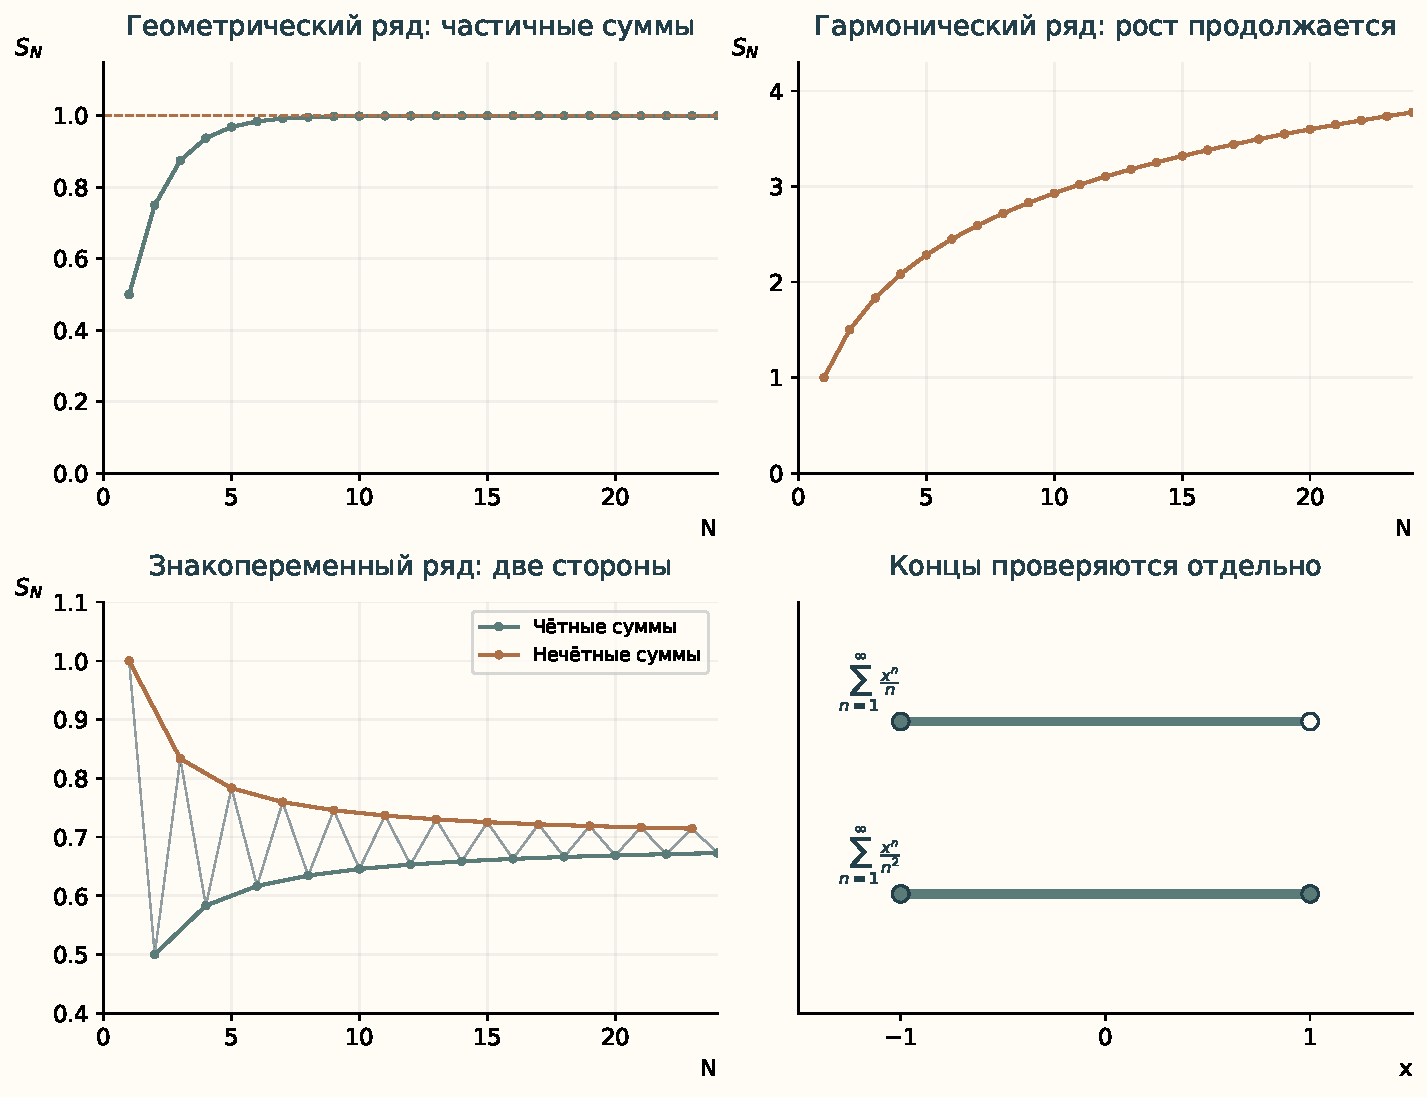
\includegraphics[width=\textwidth,height=.79\textheight,keepaspectratio]{images/atlas-series.pdf}\par\small Частичные суммы и проверка концов промежутка сходимости\end{center}\end{minipage}\par
\Needspace{7\baselineskip}\section*{Задачи}
\begingroup\setlength{\parskip}{3pt}
\noindent\begin{minipage}[t]{\linewidth}\textbf{30.1.} Для ряда \(\sum_{n=1}^\infty\dfrac1{2^n}\) выпиши первые четыре частичные суммы и найди сумму ряда.\par\end{minipage}\par
\noindent\begin{minipage}[t]{\linewidth}\textbf{30.2.} Может ли сходиться ряд с членами \(a_n=\dfrac{n}{n+1}\)?\par\end{minipage}\par
\noindent\begin{minipage}[t]{\linewidth}\textbf{30.3.} Найди сумму \(\sum_{n=1}^\infty\dfrac1{n(n+1)}\), разложив слагаемое на разность двух дробей.\par\end{minipage}\par
\noindent\begin{minipage}[t]{\linewidth}\textbf{30.4.} Исследуй сходимость рядов \(\sum\dfrac1{n^3}\), \(\sum\dfrac1{\sqrt n}\), \(\sum\dfrac1n\), \(\sum\dfrac1{n^{1{,}1}}\). Во всех суммах \(n\ge1\).\par\end{minipage}\par
\noindent\begin{minipage}[t]{\linewidth}\textbf{30.5.} Докажи сходимость \(\sum_{n=1}^\infty\dfrac1{n^2+5}\) сравнением.\par\end{minipage}\par
\par\addvspace{5pt}\begin{lrbox}{\CatFlowBox}\begin{minipage}[t]{\linewidth}
\setlength{\parskip}{5pt}\setlength{\columnsep}{4.5mm}\setlength{\intextsep}{0pt}
\begin{wrapfigure}[11]{r}{54mm}

\includegraphics[width=54mm,height=58mm,keepaspectratio]{images/unique/art-130.png}
\end{wrapfigure}
\textbf{30.6.} Докажи расходимость \(\sum_{n=1}^\infty\dfrac1{2n+1}\) сравнением.\par

\textbf{30.7.} Является ли сходимость \(\sum_{n=1}^\infty\dfrac{(-1)^{n-1}}n\) абсолютной или условной?\par

\textbf{30.8.} Исследуй абсолютную сходимость \(\sum_{n=1}^\infty\dfrac{(-1)^n}{n^2}\).\par

\textbf{30.9.} Сколько первых членов ряда \(1-\dfrac12+\dfrac13-\cdots\) достаточно сложить для ошибки не более \(0{,}01\) по оценке Лейбница? Укажи наименьшее число, которое гарантирует именно эта оценка.\par
\par\WFclear\end{minipage}\end{lrbox}%
\ifdim\dimexpr\ht\CatFlowBox+\dp\CatFlowBox\relax<64mm\dp\CatFlowBox=\dimexpr64mm-\ht\CatFlowBox\relax\fi%
\noindent\usebox{\CatFlowBox}\par\addvspace{5pt}

\noindent\begin{minipage}[t]{\linewidth}\textbf{30.10.} Используя признак Даламбера, исследуй \(\sum_{n=1}^\infty\dfrac{3^n}{n!}\) и \(\sum_{n=1}^\infty\dfrac{n!}{3^n}\).\par\end{minipage}\par
\noindent\begin{minipage}[t]{\linewidth}\textbf{30.11.} Почему признак Даламбера не решает вопрос для \(\sum\dfrac1{n^2}\)? Какой уже известный результат его решает?\par\end{minipage}\par
\noindent\begin{minipage}[t]{\linewidth}\textbf{30.12.} Найди сумму и все действительные \(x\), при которых сходится \(\sum_{n=0}^\infty(2x)^n\).\par\end{minipage}\par
\noindent\begin{minipage}[t]{\linewidth}\textbf{30.13.} Для \(\sum_{n=1}^\infty\dfrac{x^n}{n}\) найди радиус и полный промежуток сходимости, включая проверку концов.\par\end{minipage}\par
\noindent\begin{minipage}[t]{\linewidth}\textbf{30.14.} То же для \(\sum_{n=1}^\infty\dfrac{x^n}{n^2}\).\par\end{minipage}\par
\noindent\begin{minipage}[t]{\linewidth}\textbf{30.15.} Для \(\sum_{n=0}^\infty\dfrac{x^n}{n!}\) найди радиус сходимости. Вычислять сумму не требуется.\par\end{minipage}\par
\noindent\begin{minipage}[t]{\linewidth}\textbf{30.16.} Найди радиус сходимости \(\sum_{n=0}^\infty n!x^n\).\par\end{minipage}\par
\noindent\begin{minipage}[t]{\linewidth}\textbf{30.17.} В бак сначала налили 1 л воды, затем \(\dfrac12\) л, затем \(\dfrac14\) л и так далее. Найди предельный объём и сколько таких порций нужно, чтобы до него не хватало меньше \(0{,}01\) л.\par\end{minipage}\par
\noindent\begin{minipage}[t]{\linewidth}\textbf{30.18.} Длина отрезка в узоре на каждом шаге уменьшается в 3 раза; первая длина равна 9 см. Найди сумму длин всех отрезков и остаток после пяти.\par\end{minipage}\par
\noindent\begin{minipage}[t]{\linewidth}\textbf{30.19.} Докажи, что изменение конечного числа членов ряда не меняет его сходимость.\par\end{minipage}\par
\noindent\begin{minipage}[t]{\linewidth}\textbf{30.20.} Докажи линейность суммы: если \(\sum a_n=A\) и \(\sum b_n=B\), то для действительных \(\alpha,\beta\) ряд \(\sum(\alpha a_n+\beta b_n)\) сходится к \(\alpha A+\beta B\).\par\end{minipage}\par
\noindent\begin{minipage}[t]{\linewidth}\textbf{30.21.}\starmark{} Оцени сверху хвост \(\sum_{n=N+1}^\infty\dfrac1{n^2}\) без интеграла, используя сравнение с \(\dfrac1{n(n-1)}\), \(N\ge1\).\par\end{minipage}\par
\noindent\begin{minipage}[t]{\linewidth}\textbf{30.22.}\starmark{} Построй ряд, у которого \(a_n\to0\), но частичные суммы не ограничены. Докажи оба свойства.\par\end{minipage}\par
\noindent\begin{minipage}[t]{\linewidth}\textbf{30.23.}\starmark{} Найди область сходимости \(\sum_{n=1}^\infty\dfrac{(x-2)^n}{n3^n}\).\par\end{minipage}\par
\noindent\begin{minipage}[t]{\linewidth}\textbf{30.24.}\starmark{} Докажи: если степенной ряд с центром \(a\) сходится при \(x=a+2\), то он абсолютно сходится при \(x=a-1\). Обязан ли он сходиться при \(x=a-2\)?\par\end{minipage}\par
\endgroup
